%% \documentclass[landscape,final,a0paper,fontscale=0.285]{baposter}
%% \documentclass[landscape,final,a0paper,fontscale=0.4]{baposter}
%% \documentclass[landscape,a0paper,fontscale=0.35]{baposter}
\documentclass[landscape,a0paper,fontscale=0.3]{baposter}

\usepackage{calc}
\usepackage{graphicx}
\usepackage{amsmath}
\usepackage{amssymb}
\usepackage{relsize}
\usepackage{multirow}
\usepackage{rotating}
\usepackage{bm}
\usepackage{url}

\usepackage{graphicx}
\usepackage{multicol}

%% \usepackage{times}
%% \usepackage{helvet}
%\usepackage{bookman}
\usepackage{palatino}

\usepackage{lipsum}
\usepackage{jabbrv}
%% \usepackage{setspace}
\usepackage{enumitem}

\newcommand{\captionfont}{\footnotesize}

%% \graphicspath{{../figures/color/}{../figures/}}
%% \graphicspath{{images/}{../images/}}
%% \usetikzlibrary{calc}

\usetikzlibrary{arrows}
\usetikzlibrary{calc}

%%%%%%%%%%%%%%%%%%%%%%%%%%%%%%%%%%%%%%%%%%%%%%%%%%%%%%%%%%%%%%%%%%%%%%%%%%%%%%%%
%%%% Custom functions
%%%%%%%%%%%%%%%%%%%%%%%%%%%%%%%%%%%%%%%%%%%%%%%%%%%%%%%%%%%%%%%%%%%%%%%%%%%%%%%%

\newcommand{\diff}[2]{\ensuremath{\frac{d#1}{d#2}}}

%%%%%%%%%%%%%%%%%%%%%%%%%%%%%%%%%%%%%%%%%%%%%%%%%%%%%%%%%%%%%%%%%%%%%%%%%%%%%%%%
% Multicol Settings
%%%%%%%%%%%%%%%%%%%%%%%%%%%%%%%%%%%%%%%%%%%%%%%%%%%%%%%%%%%%%%%%%%%%%%%%%%%%%%%%
\setlength{\columnsep}{1.5em}
\setlength{\columnseprule}{0mm}

%%%%%%%%%%%%%%%%%%%%%%%%%%%%%%%%%%%%%%%%%%%%%%%%%%%%%%%%%%%%%%%%%%%%%%%%%%%%%%%%
% Save space in lists. Use this after the opening of the list
%%%%%%%%%%%%%%%%%%%%%%%%%%%%%%%%%%%%%%%%%%%%%%%%%%%%%%%%%%%%%%%%%%%%%%%%%%%%%%%%
\newcommand{\compresslist}{%
\setlength{\itemsep}{1pt}%
\setlength{\parskip}{0pt}%
\setlength{\parsep}{0pt}%
\raggedright%
}

\newenvironment{blockitemize}  % used when itemize takes a whole headerbox
{%
  %% \begin{minipage}{\columnwidth - 2em}
  \begin{minipage}{\columnwidth - 1em}
  \begin{itemize}
    \compresslist
}{
  \end{itemize}
  \end{minipage}
}

%%%%%%%%%%%%%%%%%%%%%%%%%%%%%%%%%%%%%%%%%%%%%%%%%%%%%%%%%%%%%%%%%%%%%%%%%%%%%%
%%% Begin of Document
%%%%%%%%%%%%%%%%%%%%%%%%%%%%%%%%%%%%%%%%%%%%%%%%%%%%%%%%%%%%%%%%%%%%%%%%%%%%%%

\begin{document}

%%%%%%%%%%%%%%%%%%%%%%%%%%%%%%%%%%%%%%%%%%%%%%%%%%%%%%%%%%%%%%%%%%%%%%%%%%%%%%
%%% Here starts the poster
%%%---------------------------------------------------------------------------
%%% Format it to your taste with the options
%%%%%%%%%%%%%%%%%%%%%%%%%%%%%%%%%%%%%%%%%%%%%%%%%%%%%%%%%%%%%%%%%%%%%%%%%%%%%%
% Define some colors

%\definecolor{lightblue}{cmyk}{0.83,0.24,0,0.12}
%% \definecolor{lightblue}{rgb}{0.145,0.6666,1}

%% \definecolor{headerfade}{rgb}{0.89,0.68,0}
%% \definecolor{headerfade}{rgb}{0.93, 0.80, 0.38}
\definecolor{headerfade}{rgb}{0.0, 0.0, 0.0}

%% \hyphenation{resolution occlusions}

\begin{poster}%
  % Poster Options
  {
  % Show grid to help with alignment
  grid=false,
  columns=4,
  % Column spacing
  colspacing=1em,
  % Color style
  bgColorOne=white,
  bgColorTwo=white,
  borderColor=headerfade,
  headerColorOne=black,
  headerColorTwo=headerfade,
  headerFontColor=white,
  boxColorOne=white,
  boxColorTwo=headerfade,
  % Format of textbox
  textborder=roundedleft,
  % Format of text header
  eyecatcher=true,
  headerborder=closed,
  headerheight=0.17\textheight,
%  textfont=\sc, An example of changing the text font
  headershape=roundedright,
  headershade=shadelr,
  headerfont=\Large\bf, %Sans Serif
  %% headerfont=\Large\bf\textsc, %Sans Serif
  textfont={\setlength{\parindent}{1.5em}},
  boxshade=plain,
%  background=shade-tb,
  background=plain,
  linewidth=2pt
  }
  % Eye Catcher
  {
    \begin{tabular}{c}
      \relax\\
      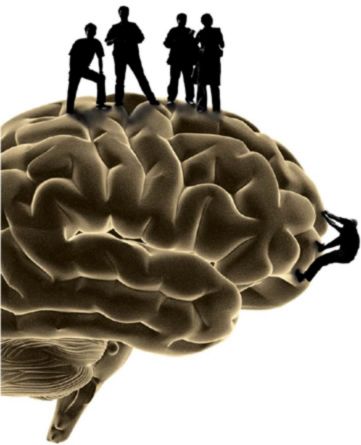
\includegraphics[height=13em]{brain.png}
    \end{tabular}
  }
  % Title
  {
    %% \textbf{\textsc{Heterogeneity and Noise in Population Coding}}\vspace{0.5em}
    %% \textbf{\textsc{Heterogeneity Increases Information Transmission\\[0.5em]
    %%     in Neuronal Populations}}\vspace{0.5em}
    \textbf{Biologically realistic supervised deep learning\\in spiking LIF neurons}\vspace{0.5em}
  }
  % Authors
  {
    Eric Hunsberger, Chris Eliasmith\\[0.2em]
    \{ehunsber,celiasmith\}@uwaterloo.ca\\[0.4em]
    %% Centre for Theoretical Neuroscience, University of Waterloo (\url{http://ctn.uwaterloo.ca})
  }
  % University logo
  {% The makebox allows the title to flow into the logo, this is a hack because of the L shaped logo.
    %% 
\includegraphics[height=9.0em]{ctn.png}
    \begin{tabular}{cc}
      \relax\\
      
\includegraphics[height=6.0em]{uwaterloo.png} &
      
\includegraphics[height=5.0em]{ctn.png}\\
      \multicolumn{2}{c}{
        
\includegraphics[height=5.0em]{cnrg.png}}
    \end{tabular}
  }

%%%%%%%%%%%%%%%%%%%%%%%%%%%%%%%%%%%%%%%%%%%%%%%%%%%%%%%%%%%%%%%%%%%%%%%%%%%%%%
%%% Now define the boxes that make up the poster
%%%---------------------------------------------------------------------------
%%% Each box has a name and can be placed absolutely or relatively.
%%% The only inconvenience is that you can only specify a relative position
%%% towards an already declared box. So if you have a box attached to the
%%% bottom, one to the top and a third one which should be in between, you
%%% have to specify the top and bottom boxes before you specify the middle
%%% box.
%%%%%%%%%%%%%%%%%%%%%%%%%%%%%%%%%%%%%%%%%%%%%%%%%%%%%%%%%%%%%%%%%%%%%%%%%%%%%%
    %
    % A coloured circle useful as a bullet with an adjustably strong filling
    \newcommand{\colouredcircle}{%
      \tikz{\useasboundingbox (-0.2em,-0.32em) rectangle(0.2em,0.32em);
        \draw[draw=black,fill=headerfade,line width=0.03em] (0,0) circle(0.18em);}}

    %%%%%%%%%%%%%%%%%%%%%%%%%%%%%%%%%%%%%%%%%%%%%%%%%%%%%%%%%%%%%%%%%%%%%%%%%%%%%%%%

    \headerbox{Motivation}{name=intro,column=0,row=0}{
      \noindent
      Backprop (BP) is not biologically plausible \cite{Bengio2015}:

      \noindent
      \begin{itemize}
        \compresslist
        \item Error pathway is purely linear
        \item Error pathway uses present derivatives of forward neurons
        \item Error pathway uses weights symmetric to those of forward pathway (aka. tied weights)
        \item Forward and error pathways synchronous
        \item Treats neurons as non-spiking, differentiable
        %% \item Where do the output targets come from?
      \end{itemize}
    }


    \headerbox{Feedback Alignment (FA)}{name=fa,column=0,below=intro}{
      \noindent
      A more biologically plausible alternative to backpropagation
      developed by \cite{Lillicrap2016}:
      \begin{itemize}
        \compresslist
        \item Uses random feedback weights, instead of symmetric ones
        \item Forward weights in later layers ``align'' so that feedback
          weights carry useful information
        \item Hidden neurons pushed towards random targets,
          but only when there is error (c.f. unsupervised learning)
        \item Hidden neurons pushed in different directions depending on
          ``type'' of error (i.e. vector difference between output and target)
      \end{itemize}

      %% \vspace{-1em}
      \noindent
      \begin{center}
        \tikzstyle{line} = [draw]

\begin{tabular}{ccc}
  Backprop & FA & Our model \\
\begin{tikzpicture}[->,>=stealth',auto,node distance=1cm,
    thick,circnode/.style={circle,draw,inner sep=2}]
  \node[circnode] (h) {$h$};
  \node[circnode] (d) [right of=h, node distance=1.5cm] {$\delta$};
  \node[] (ah) [above of=h] {};
  \node[] (bh) [below of=h] {};
  \path[line] (bh) -- node [right] (W) {$W$} (h);
  \path[line] (h) -- (ah);
  \node[] (ad) [above of=d] {};
  \node[] (bd) [below of=d] {};
  \path[line] (ad) -- (d);
  \path[line] (d) -- node [right] {$W^T$} (bd);
  \path[line] (h) to [out=45,in=135] node {$h'$} (d);
  \path[line] (d) to (W);
\end{tikzpicture} &
\begin{tikzpicture}[->,>=stealth',auto,node distance=1cm,
    thick,circnode/.style={circle,draw,inner sep=2}]
  \node[circnode] (h) {$h$};
  \node[circnode] (d) [right of=h, node distance=1.5cm] {$\delta$};
  \node[] (ah) [above of=h] {};
  \node[] (bh) [below of=h] {};
  \path[line] (bh) -- node [right] (W) {$W$} (h);
  \path[line] (h) -- (ah);
  \node[] (ad) [above of=d] {};
  \node[] (bd) [below of=d] {};
  \path[line] (ad) -- (d);
  \path[line] (d) -- node [right] {$B$} (bd);
  %% \path[line] (h.north) to [out=45,in=45] node {$h'$} (W);
  \path[line] (h.north) .. controls +(right:5mm) and +(up:5mm)
                        .. node {$h'$} (W.north east);
  \path[line] (d) to (W);
\end{tikzpicture} &
\begin{tikzpicture}[->,>=stealth',auto,node distance=1cm,
    thick,circnode/.style={circle,draw,inner sep=2}]
  \node[circnode] (h) {$h$};
  \node[circnode] (d) [right of=h, node distance=1.5cm] {$e$};
  \node[] (ah) [above of=h] {};
  \node[] (bh) [below of=h] {};
  \path[line] (bh) -- node [right] (W) {$W$} (h);
  \path[line] (h) -- (ah);
  \node[] (ad) [above of=d] {};
  \node[] (bd) [below of=d] {};
  \path[line] (ad) -- (d);
  \path[line] (d) -- (bd);
  %% \path[line] (h.north east) to [out=45,in=45] node {$h'$} (W);
  \path[line] (h.north) .. controls +(right:5mm) and +(up:5mm)
                        .. node {$h'$} (W.north east);
  \path[line] (d) to node {$B$} (W);
\end{tikzpicture}
\end{tabular}

      \end{center}

      \noindent
      \textbf{Limitations:}
      \begin{itemize}
        \compresslist
        \item Feedforward neurons are sigmoidal, stochastically spiking
        \item Feedback neurons are sigmoidal, non-spiking,
          allow negative firing rates
      \end{itemize}
    }

    \headerbox{References}{name=references,column=0,above=bottom}{
      \scriptsize
      \renewcommand{\refname}{\vspace{-0.8em}}
      \bibliographystyle{jabbrv_ieeetr}
      \bibliography{/media/dropbox/papers/bib/library}
    }

    \headerbox{Spiking Results}{name=online,column=1,span=2,above=bottom}{
      %% \vspace{-1em}
      \begin{center}
        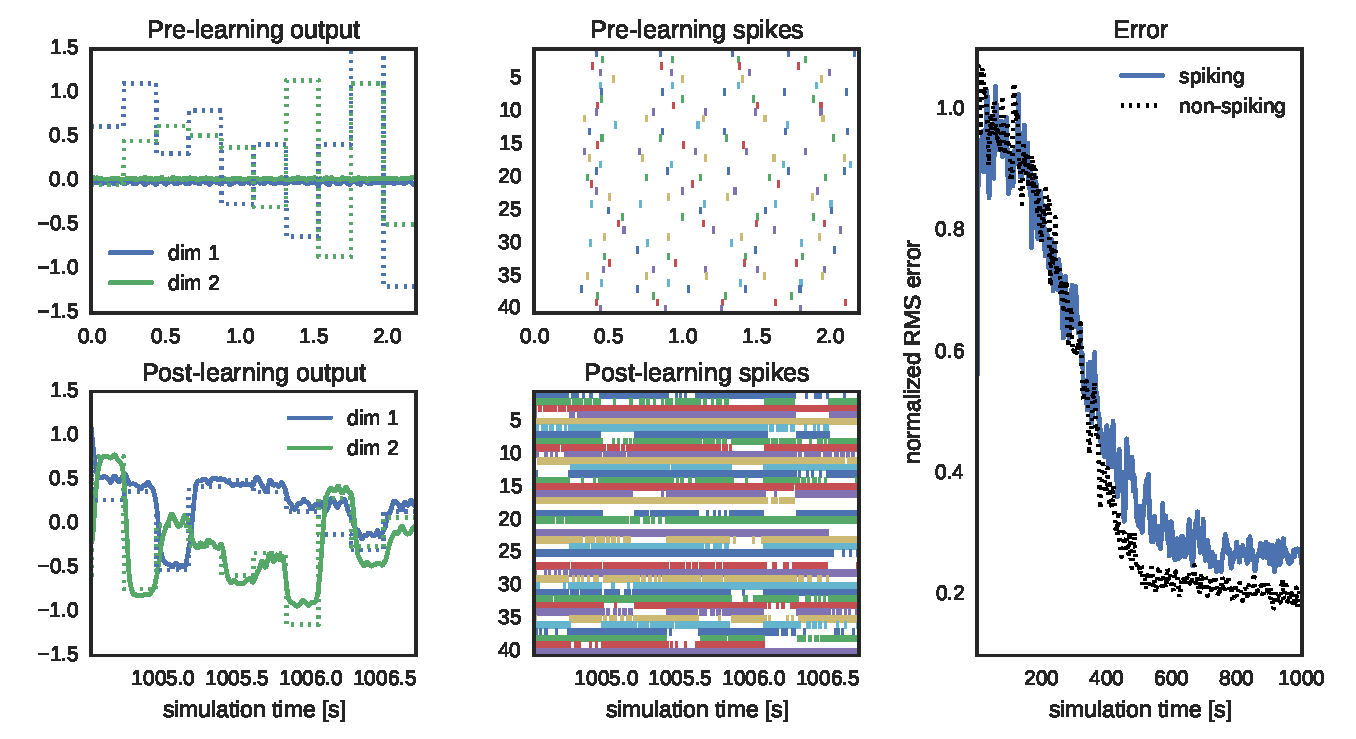
\includegraphics[width=\columnwidth, clip=true, trim=0mm 0mm 0mm 3mm]{figures/online.pdf}
        %% \includegraphics[width=\columnwidth]{figures/online2.pdf}
      \end{center}
      \vspace{-2.5em}

      \begin{multicols}{2}
      \noindent
      Here, the fully spiking algorithm learns a deep network.
      Before learning, the network has no output, and spikes in the second
      hidden layer (shown) are sparse and independent of the input.
      After learning, the network produces the target output,
      and hidden-layer neurons are selective to different inputs.
      The accuracy is comparable to the non-spiking network.
      \end{multicols}
    }

    \headerbox{Solution}{name=solution,column=1,above=online}{
      \noindent
      \vspace{-1em}
      \begin{itemize}
        \compresslist
        \item Use population coding to transmit final-layer error backwards.
          This allows the encoding of negative errors.
        %% \item Use random projection of error to adjust forward weights
        \item Use spiking LIF neurons throughout,
          with a surrogate derivative for learning
      \end{itemize}

      \noindent
      \textbf{Validation problem:}
      \vspace{-0.5em}
      \begin{itemize}
        \compresslist
        \item Data: Linear mapping from 30-D to 10-D, normally distributed.
          Nontrivial to learn with nonlinear neurons.
        \item Network: Two hidden layer (30-80-80-10) network.
          Demonstrates ability to learn deep networks.
          Spiking network has 3 ms alpha synapses between layers.
        \item Training: Trained both non-spiking and spiking versions.
          For spiking network, each stimulus is presented for 220 ms.
      \end{itemize}
    }

    \headerbox{Non-spiking Results}{name=offline,column=2,above=online}{
      %% \vspace{-1em}
      \begin{center}
        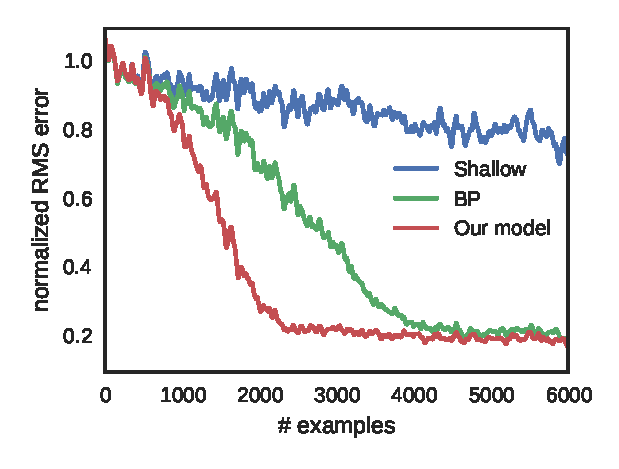
\includegraphics[width=\columnwidth, clip=true, trim=0mm 0mm 0mm 4.5mm]{figures/offline.pdf}
        %% \includegraphics[width=\columnwidth]{figures/offline2.pdf}
      \end{center}
      \vspace{-2em}
      Both BP and our model are able to solve the problem
      using rate-based LIF neurons.
      Because the initial forward weights are small,
      our model learns quicker than BP because it has larger feedback weights.
    }

    \headerbox{LIF neuron derivatives}{name=lifderivative,column=3,row=0}{
      \noindent
      The leaky integrate-and-fire (LIF) neuron dynamics:
      \begin{align}
        \tau_{RC} \diff{V}{t} &= -V + J(t)
        \nonumber
      \end{align}
      Spikes when $V > 1$, then $V = 0$ for $t_{ref}$ seconds.

      The instantaneous firing rate in Hertz is:
      \begin{align}
        h(u) = \left(t_{ref} + \tau_{RC} \log\left(1 + \frac{1}{\max(u - 1, 0)}\right)\right)^{-1}
        \nonumber
      \end{align}

      \begin{itemize}
        \compresslist
        \item Problem: $h' \to \infty$ as $u \to 1^+$
        \item Solution: Replace $h'$ with surrogate derivative function
          (derivative of IF neuron with refractory period)
        \item Derivative no longer matches nonlinearity, but learning still works
      \end{itemize}

      \begin{center}
        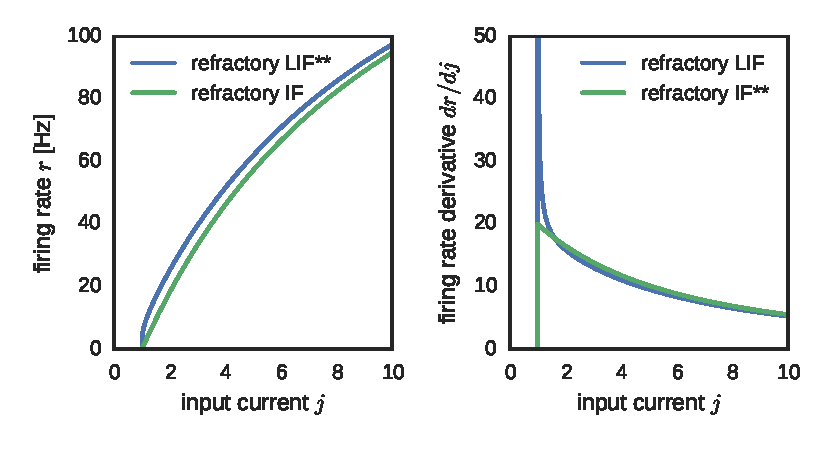
\includegraphics[width=\columnwidth, clip=true, trim=3mm 6mm 3mm 4mm]
                        {figures/lifderivative.pdf}
      \end{center}

      \vspace{-1.5em}
      \begin{flushright}
        \scriptsize
        ** used in model
      \end{flushright}
    }

    \headerbox{Discussion}{name=conclusions,column=3,below=lifderivative,above=bottom}{
      \noindent
      \begin{blockitemize}
        \compresslist
        %% \item Extended FA algorithm to fully spiking network,
        %%   using more realistic LIF neurons instead of sigmoid neurons.
        \item Fully-spiking FA-based network,
          using more realistic LIF neurons instead of sigmoid neurons
        \item Population coding used to transmit negative errors
        \item Surrogate derivative used for the LIF neurons when learning.
          Used derivative of refractory IF, but plain IF derivative
          (i.e., step function) also works.
        \item Network includes synaptic delays. Each stimulus must be presented
          long enough for the network to learn from it,
          but short enough to expose the network to a variety of stimuli.
      \end{blockitemize}
    }

    %% \headerbox{Future work}{name=future,column=3,below=conclusions}{
    %%   \noindent
    %%   \begin{blockitemize}
    %%     \compresslist
    %%     \item Compare more carefully with backprop, DTP, and unsupervised rules.
    %%       How does the learned representation vary?
    %%     \item Combine superived and unsupervised rules in the same layers
    %%   \end{blockitemize}
    %% }


    % Panel idea: alternatives: Unsupervised and DTP
    %   Unsupervised: Can only learn based on input statistics, ignorant of
    %   function being learned. For example, if the desired function depends
    %   on only some of the input dimensions, not able to take advantage.
    %   DTP: Need two phases, one for adjusting forward connections based on
    %   current training image using backwards connections, and one for
    %   adjusting backwards connections using variations on training images
    %   through forwards connections. Guergiuev does this with compartmental
    %   neurons.

\end{poster}
\end{document}
